\documentclass[12pt,a4paper]{article}
\usepackage[T1]{fontenc}
\usepackage[utf8x]{inputenc}
\usepackage[french]{babel}
\usepackage{lmodern}
\usepackage{graphicx}
\usepackage{enumitem}
\usepackage{rotating}
\usepackage{dirtree}
\usepackage{subcaption}
\usepackage{microtype}
\usepackage{listings}
\usepackage{hyperref}

\title{Conception d'une application web de réservation\\[3mm] \normalsize{\it Laboratoire de technologie web}}
\author{Christophe Simon \\ Guillaume de Moffarts}
\date{\today}
\setlength\topmargin{-10mm}
\setlength\headheight{0mm}
\setlength\textheight{24cm}
\setlength\oddsidemargin{-0.5cm}
\setlength\textwidth{16.5cm}
\setlength{\parskip}{3mm}
\setlength{\parindent}{0mm}
\usepackage{xcolor}

\lstdefinelanguage{php}
{morekeywords=[1]{class,function,private,return,if,else,for,throw,new,null,while,for,foreach,as},
morekeywords=[2]{},
morekeywords=[3]{echo,Exception,exit,empty,header,isset,serialize,unserialize,count,array_push,array,die,sprintf, include},
morekeywords=[4]{\$this,\$_POST,\$_SESSION},
morekeywords=[5]{mysqli_query,mysqli_num_rows,mysqli_fetch_assoc,mysqli_connect,mysqli_close,mysqli_stmt_init,mysqli_stmt_prepare,mysqli_stmt_bind_param,mysqli_stmt_execute,mysqli_insert_id,mysqli_error,mysqli_connect_error},
morestring=[b]{"},
morestring=[b]{'},
morecomment=[l]{//},}

\lstdefinelanguage{CSS}
{morekeywords=[1]{color,border,text,decoration,margin,padding,left,top,right,background,font,size,weight,float, width, height, display, position, cursor, bottom, opacity, radius, content, family, transition, webkit, transform, max, overflow},
morekeywords=[2]{first,child,nth,of,type,letter,selection},
morekeywords=[3]{h1,p,div,tr,td},
morekeywords=[4]{},
morekeywords=[5]{},
sensitive,
morecomment=[s]{/*}{*/},}

\lstset{
    extendedchars=\true,
    inputencoding=utf8x,
    basicstyle=\fontfamily{pcr}\selectfont\scriptsize\color{black},
    keywordstyle=[1]\color{blue}\bfseries, % style for keywords
    keywordstyle=[3]\color[rgb]{0,0.6,0}\bfseries, % style for keywords
    keywordstyle=[4]\color[rgb]{0.6,0,0}\bfseries, % style for keywords
    keywordstyle=[5]\color[rgb]{0,0.2,0}\bfseries, % style for keywords
    stringstyle=\color[rgb]{0.6,0.47,1}, %style between " "
    commentstyle=\color[rgb]{0.3,0.7,0.3},
    %numbers=left, % where to put the line-numbers
    %numberstyle=\tiny, % the size of the fonts that are used for the line-numbers
    showspaces=false, % show spaces adding particular underscores
    showstringspaces=false, % underline spaces within strings
    showtabs=false, % show tabs within strings adding particular underscores
    frame=single, % adds a frame around the code
    tabsize=2, % sets default tabsize to 2 spaces
    rulecolor=\color{black},
    captionpos=b, % sets the caption-position to bottom
    breaklines=true, % sets automatic line breaking
    breakatwhitespace=false,
    frame={}
}

\usepackage{listingsutf8}
\usepackage{libertine}
\newcommand{\file}[1]{"C:/wamp64/www/BryanAir/#1"}

\begin{document}
	\maketitle
	\section*{Introduction}
		Dans le cadre du laboratoire de Technologie web, nous avons réaliser une application web dont le but est de réserver des billets d'avion. Cette application doit suivre le design pattern MVC (Model View Controler).

		Nous avons choisis comme idée de réaliser une caricature de la compagnie aérienne Ryanair, que nous avons appeler BryanAir. Le style de notre application à été inspirer du site officiel de la compagnie.

		Dans ce rapport, vous allez trouver des explications sur le fonctionnement normal et erroné de l'application. Vous y trouverez un diagramme de séquence pour imager cela.


	\section{Description du site}
		Il y a tout d'abord une page d'accueil (figure~\ref{fig:home}) qui permet de se rediriger vers une section pour effectuer la réservation d'un vol.
		\begin{figure}
			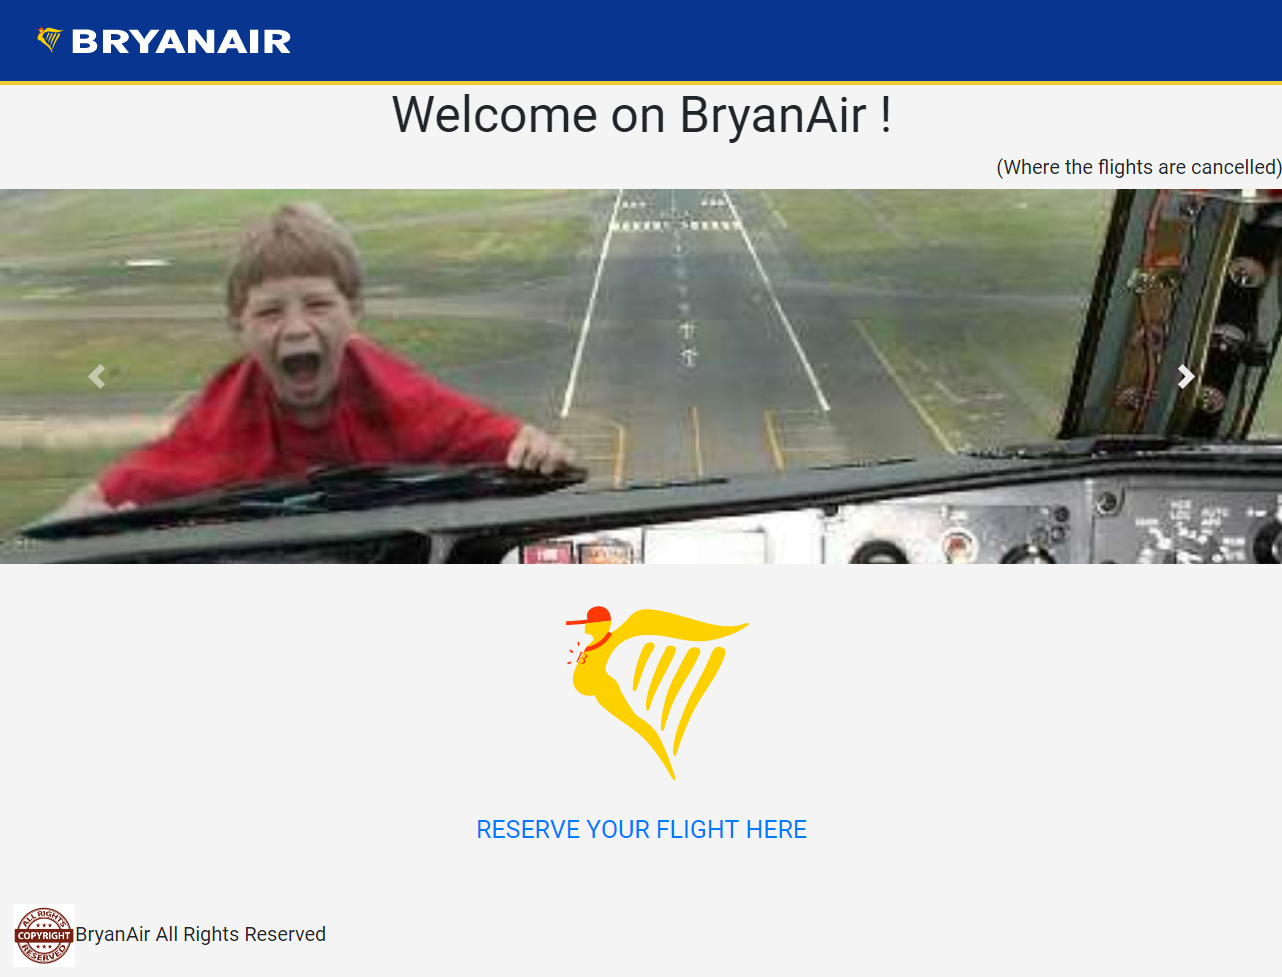
\includegraphics[width=\textwidth]{home.png}
			\caption{Page d'accueil}
			\label{fig:home}
		\end{figure}

		Sur la première page de réservation (figure~\ref{fig:res1}), on peut réserver un ou plusieurs billets. Il faut donner l'aéroport de départ et d'arrivée, si on veut réserver un billet aller simple ou aller retour, le nombre de passager, l'adresse email et si on désire une assurance annulation ou pas.
		\begin{figure}
      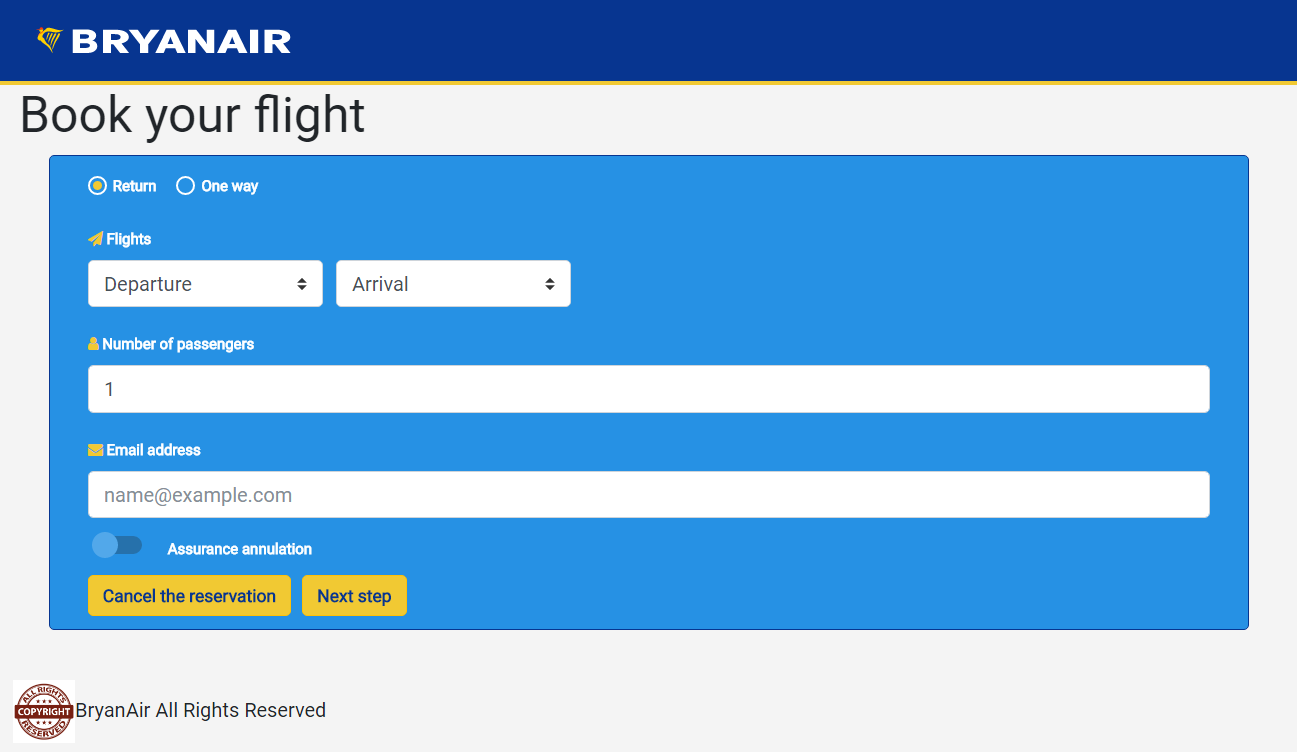
\includegraphics[width=\textwidth]{Reservation.png}
			\caption{Réservation étape 1}
			\label{fig:res1}
		\end{figure}

		La deuxième étape de réservation (figure~\ref{fig:res2}) consiste a enregistrer les informations pour chaque passager tel que le nom, le prénom et l'age.
		\begin{figure}
      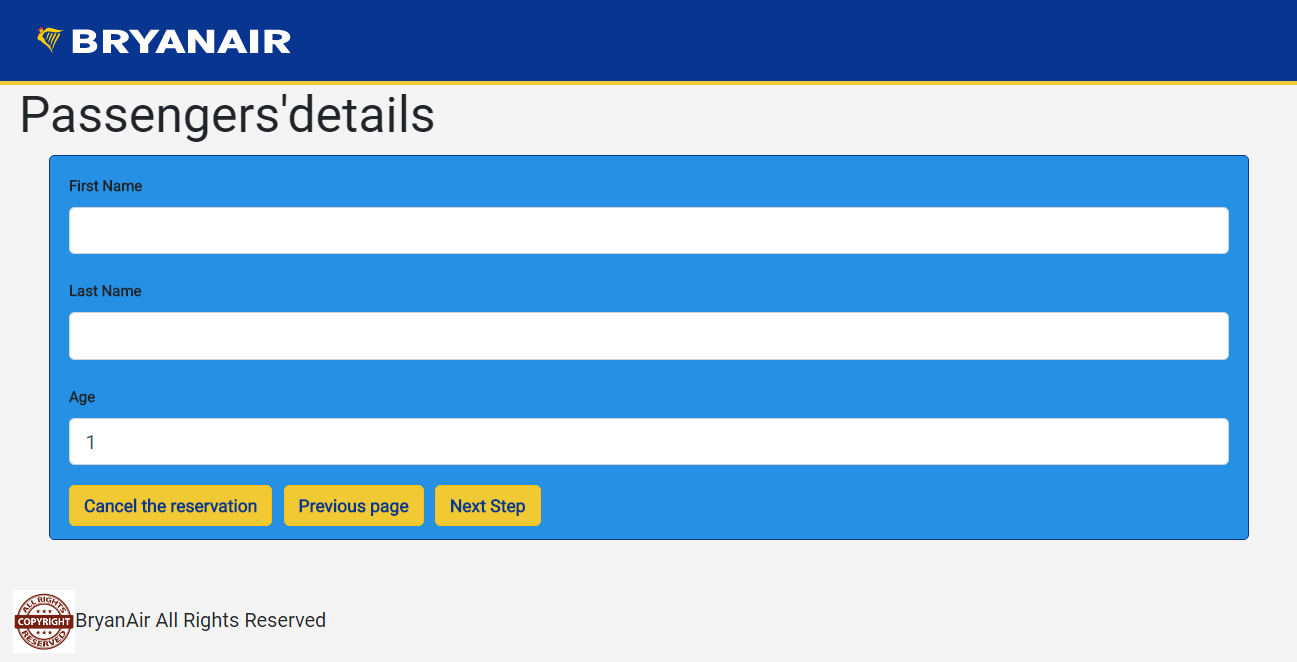
\includegraphics[width=\textwidth]{Detail.png}
			\caption{Réservation étape 2}
			\label{fig:res2}
		\end{figure}

		Une fois tous les passagers enregistrés, on arrive sur une page de confirmation (figure~\ref{fig:conf}) ou vous avez le choix de confirmer ou d'annuler.

		\begin{figure}
      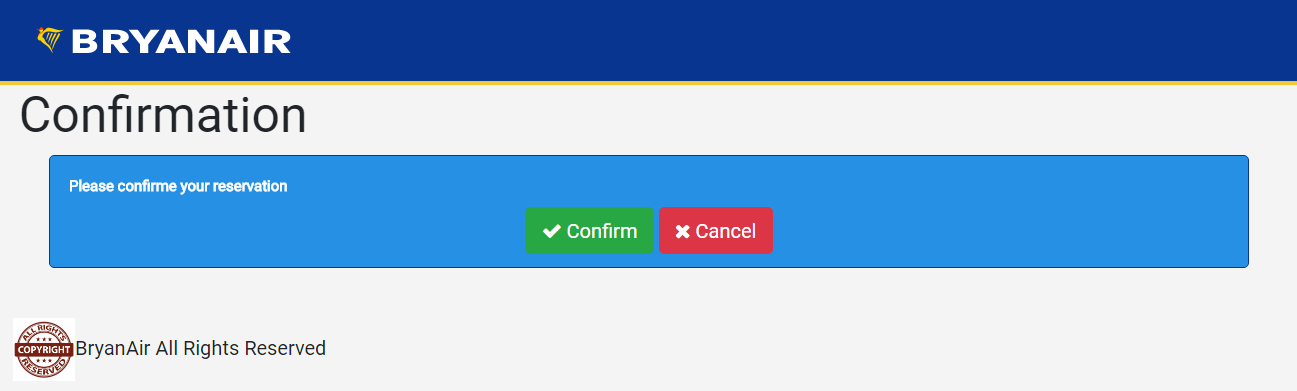
\includegraphics[width=\textwidth]{Confirmation.png}
			\caption{Confirmation}
			\label{fig:conf}
		\end{figure}
		Une fois la réservation confirmée, on arrive sur une page récapitulant la commande (figure~\ref{fig:recap}) avec le prix a payer.
		\begin{figure}
      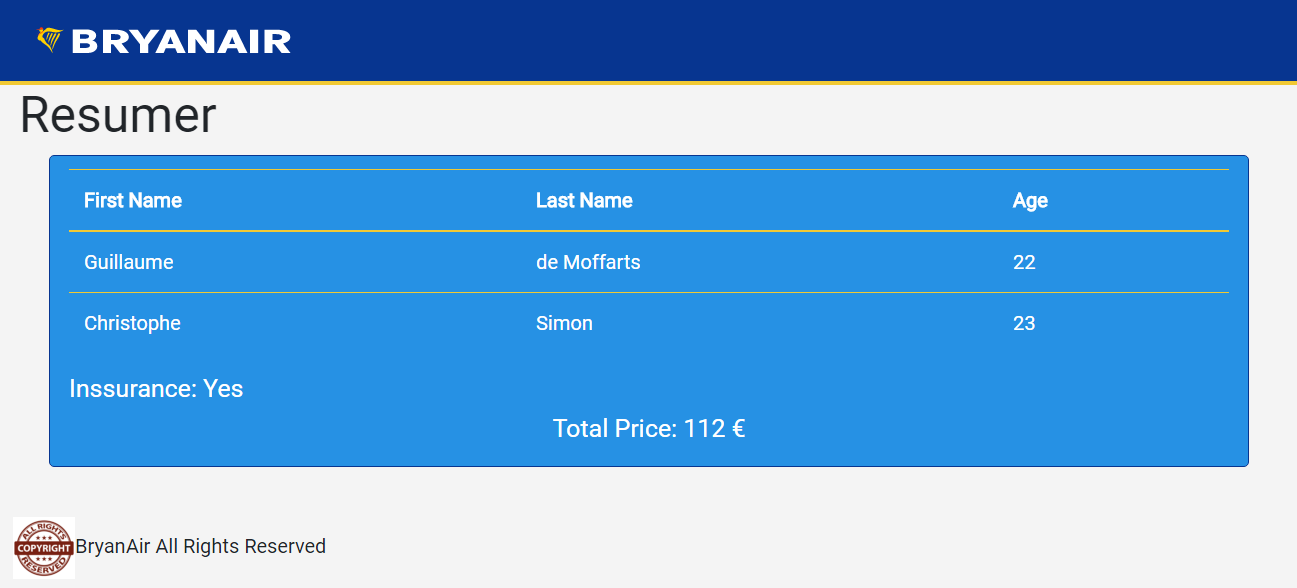
\includegraphics[width=\textwidth]{Resumer.png}
			\caption{Récapitulatif}
			\label{fig:recap}
		\end{figure}

		Enfin, il y a une page d'administration (figure~\ref{fig:admin}) ou on peut voir, éditer ou supprimer les passager pour chaque vol. Cette page ne devant ètre accessible du public, on y accède uniquement via \url{http://localhost/BryanAir/admin}.

		\begin{figure}
      \includegraphics[width=\textwidth]{admin.png}
			\caption{Page admin}
			\label{fig:admin}
		\end{figure}

	\section{Fonctionnement}
		Dans cette section, vous retrouvez les explications sur le fonctionnement des différentes partie de l'application, tel que la redirection d'URL, les réservation et la page d'administration et les templates html.
		\subsection*{Redirection}
		La conception de l'application est basé sur le design pattern MVC. Nous avons donc un routeur, des contrôleurs et des views. Le routeur redirige vers le contrôleur adéquate qui va vérifier les informations venant des formulaire, charger et enregistrer les modèles dans la base de donnée. Le contrôleur va ensuite afficher la page.

		Lorsque qu'on veux accéder a une page, il suffit d'utiliser l'URL suivante \url{localhost/BryanAir/} suivit du nom de la page a accéder. Cette URL est rediriger vers \url{localhost/Bryanair?page=<nom_de_page>} car le routeur a besoin d'une variable \texttt{GET["page"]} pour pouvoir rediriger vers le bon controleur. Nous avons fait ce choix pour qu'il soit plus facile d'accéder aux différentes pages. Cette redirection est configurer dans le fichier \texttt{.htacces}.

		\subsection*{Templates}
		Pour faciliter la construction des vues, nous avons utiliser un sytème de templates html. Nous avons plassé des balises comme suit \texttt{\$balise\$} dans nos pages html. Celle-ci vont etre remplacer par le contrôleur. La fonction \texttt{buildHTML} dans le fichier \texttt{utils.php} construit d'abord la page en concaténant quartes fichiers HTML. Trois de ces fichier sont commun pour toute les vues, il y'a a le \texttt{head.html}, le \texttt{header.html} et le \texttt{footer.html}.  Entre ces deux dernier, la vue propre a la page est ajouté.
		On remplace ensuite toute les balise, grâce a du regex, par des bouts d'HTML construit par le contrôler. Cette fonction prend en paramètre un liste de clef valeurs, les clefs correspond aux mots dans les balises de l'HTML et les valeur contienne donc le contenu a remplacer.

		Cette méthode permet de faciliter grandement la création des vues. En effet, il ne sera pas nécésaire de copier dans tous les fichier html un bout de code commun a toute les pages. Cette méthodes permet aussi de bien séparer la partie vu de la partie controleur.

		\subsection{Réservation}
      Tous d'abord, en cliquant sur le bouton réservation de la page d'acceuil, le controleur (controle\_reservation.php) charge la liste de tous les aéroport présent dans la base de donées. Le contrôleur va ensuite contruire la page de réservation grace a cette liste.

			Lorsque l'utilisateur valide la première page de réservation (figure~\ref{fig:res1}), un contrôleur (controleur\_detail.php) vérifie tout d'abord les données venant du \texttt{POST}. En effet si on passe bien par le formulaire, il ne devrais pas avoir de problème mais on peut tout a fait utilisé un outil tel que curl pour envoyer n'importe quel requète POST au serveur ou tout simplement en changeant l'html dans l'inspecteur du navigateur, on peut envoyer du text au lieu d'un entier. Il faut donc bien vérifier que toutes les données du \texttt{POST} nécessaire au contrôleur on bien été définies et sont de type correcte. Par exemple, la variable contenant le nombre de passager doit pouvoir ètre convertit en un entier. Si un problème survient dans la vérification des variables , vous etes redirigez vers la page précédentes avec un message d'erreur sur le haut de celle ci (figure~\ref{fig:error}. Si la vérification a réussie, Le controleur cherche dans la base de donnée les numéros de vols (aller/retour) et le nombre de place restantes. Si il n'y a plus de place pour un des vols ou qu'il ne trouve pas de vol pour les aéroport sélectionner, on aura un message d'erreur comme décrit précédement. Toutes ces informations sont utilisées pour pour instanttier un objet de type \texttt{Reservation} et en définir l'état. Le controleur va ensuite construire la page HTML (detail.html) grace a la fonction expliqué dans les section précédente.
			\begin{figure}
        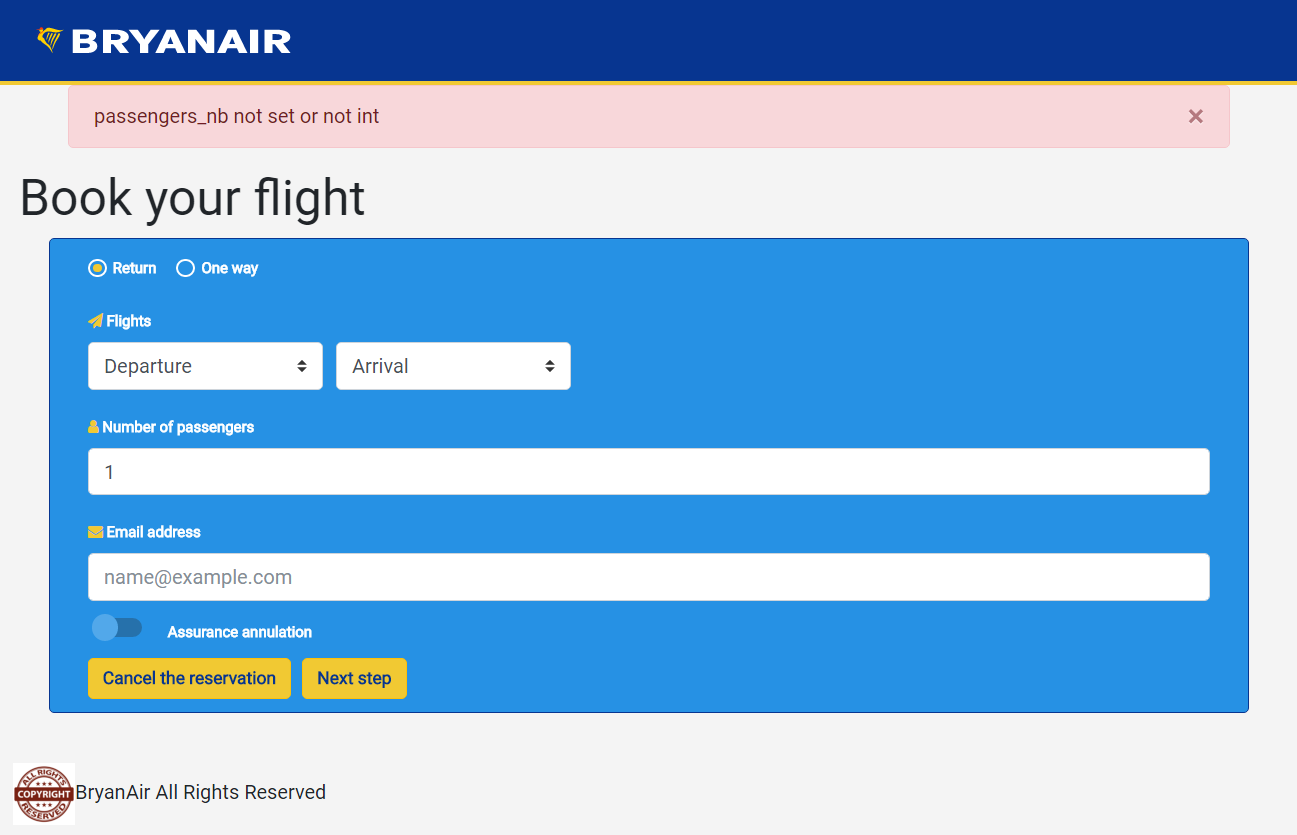
\includegraphics[width=\textwidth]{Error.png}
				\caption{Message d'erreur}
				\label{fig:error}
			\end{figure}


			Nous somme maintenant a la deuxième étapes de la réservations (figure~\ref{fig:res2}) où il faut encoder un a un les informations sur les passagers. Comme pour la première étapes, un contrôleurs (controleur\_nextpassenger.php) vérifie les informations de la variable \texttt{HTTP POST}, le même systéme d'erreur est aussi d'application. Une fois la vérification passée, le contrôleur instancie un objet de type \texttt{Client} dont l'état est définit pas les informations entrées dans le formulaire. Cet objet client est ensuite ajouter dans la liste de client de l'objet réservation. Si il y a encore des passager a enregistrer, le contrôleur contruit la même page html que précédemment pour enregistrer un nouveau passager. Si tous les passager sont enregistré, le contrôleur construit la page de confirmation (confirmation.html).

			Une fois arriver sur la page de confirmation (figure~\ref{fig:conf}), on a le choix entre confirmer la réservation ou de l'annuler. Si la réservation est annulée, on est redirigé vers la page d'accueil et les l'objet réservation avec la liste des client est supprimé. Si on confirme la réservation, un contréleur (controleur\_confirmation.php) vérifie si au moins un des passagers est bien majeurs. Si ce n'est pas le cas, le système d'erreur affiche un message (figure~\ref{fig:ageError}), il faudra ré-encoder les informations des passagers. Si il y a bien au moins une personne majeur, le contrôleur enregistre les clients et réservations dans la basse de données et va ensuite nous rediriger vers une page résumant la commande(figure~\ref{fig:recap}).

			\begin{figure}
        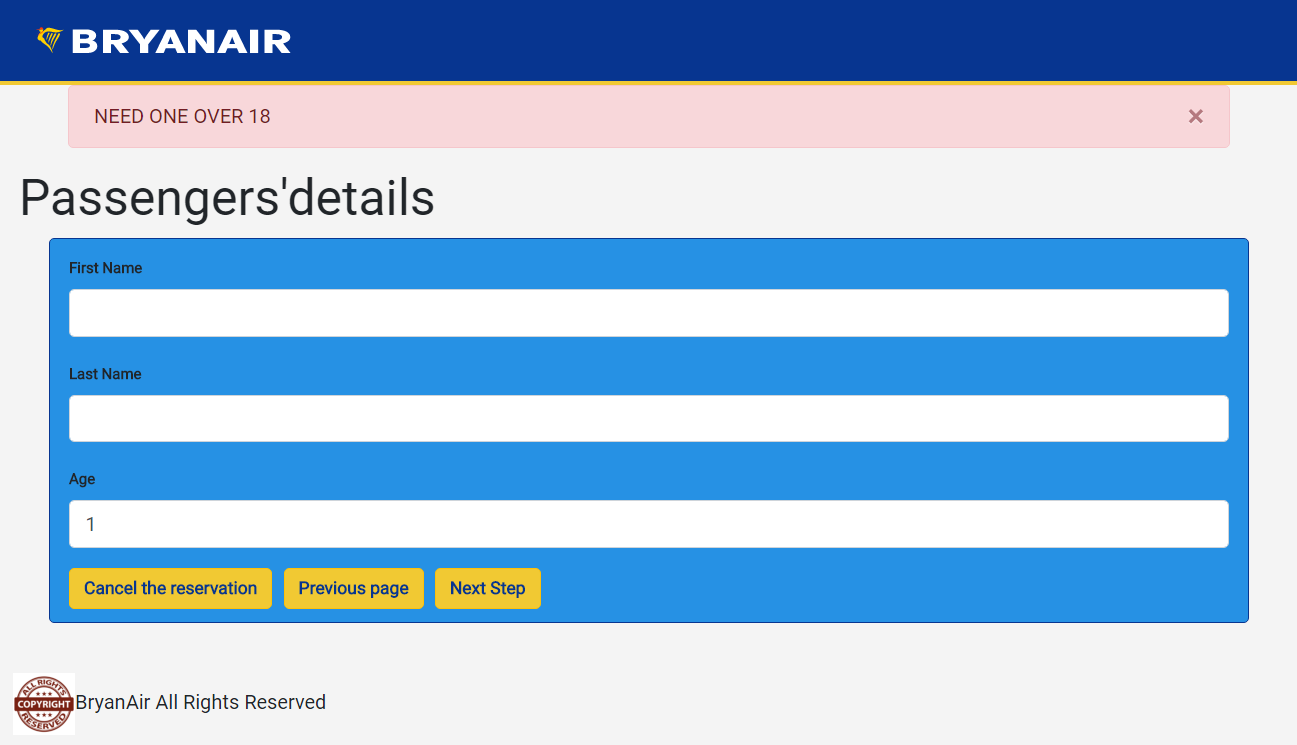
\includegraphics[width=\textwidth]{ageError.png}
				\caption{Erreur de majorité}
				\label{fig:ageError}
			\end{figure}

			Le contrôleur (controleur\_resumer.php) permettant d'afficher cette page vas tout d'abord construire un tableau html, avec tout les passagers  de la réservation, grâce a l'objet réservation. Cet objet se charge aussi de calculer le prix total a payer en se basant sur le nombre de passager, si il on prix un vol aller retour ou aller simple et enfin, si une assurance annulation est prise. Le contrôleur vas ensuite construire la page avec toute ces information.

		\subsection{Admin}
			En allant sur la page admin, le contrôleur (controler\_admin.php) charge depuis la base de donnée tout les vols ainsi que les passager pour chacun d'eux. Il en fait un tableau html représantant toute ces donnée puis construit la page html (admin.html).

	\section*{Conclusion}

  \pagebreak
  \appendix
  \section{Modèles}
    \subsection{Client.php}
    \lstinputlisting[language=php]{\file{models/Client.php}}
    \subsection{Flight.php}
    \lstinputlisting[language=php]{\file{models/Flight.php}}
    \subsection{Reservation.php}
    \lstinputlisting[language=php]{\file{models/Reservation.php}}
\section{templates}
  \subsection{home.html}
  \lstinputlisting[language=html]{\file{templates/home.html}}
  \subsection{reservation.html}
  \lstinputlisting[language=html]{\file{templates/reservation.html}}
  \subsection{detail.html}
  \lstinputlisting[language=html]{\file{templates/detail.html}}
  \subsection{confirmation.html}
  \lstinputlisting[language=html]{\file{templates/confirmation.html}}
  \subsection{resumer.html}
  \lstinputlisting[language=html]{\file{templates/resumer.html}}
  \subsection{admin.html}
  \lstinputlisting[language=html]{\file{templates/admin.html}}
  \subsection{head.html}
  \lstinputlisting[language=html]{\file{templates/head.html}}
  \subsection{header.html}
  \lstinputlisting[language=html]{\file{templates/header.html}}
  \subsection{footer.html}
  \lstinputlisting[language=html]{\file{templates/footer.html}}
  \subsection{admin.html}
  \lstinputlisting[language=html]{\file{templates/admin.html}}

\section{Controlers}
  \subsection{controler\_home.php}
  \lstinputlisting[language=php]{\file{controler_home.php}}
  \subsection{controle\_reservation.php}
  \lstinputlisting[language=php]{\file{controler_reservation.php}}
  \subsection{controler\_detail.php}
  \lstinputlisting[language=php]{\file{controler_detail.php}}
  \subsection{controler\_nextpassenger.php}
  \lstinputlisting[language=php]{\file{controler_nextpassenger.php}}
  \subsection{controler\_confirmation.php}
  \lstinputlisting[language=php]{\file{controler_confirmation.php}}
  \subsection{controler\_resumer.php}
  \lstinputlisting[language=php]{\file{controler_resumer.php}}
  \subsection{controler\_admin.php}
  \lstinputlisting[language=php]{\file{controler_admin.php}}
  \subsection{controler\_update.php}
  \lstinputlisting[language=php]{\file{controler_update.php}}
  \subsection{controler\_delete.php}
  \lstinputlisting[language=php]{\file{controler_delete.php}}
  \subsection{controler\_404.php}
  \lstinputlisting[language=php]{\file{controler_404.php}}

\section{Other}
  \subsection{.htaccess}
  \lstinputlisting[language={}]{\file{.htaccess}}
  \subsection{index.php}
  \lstinputlisting[language=php]{\file{index.php}}
  \subsection{utils.php}
  \lstinputlisting[language=php]{\file{utils.php}}
  \subsection{style.css}
  \lstinputlisting[language=css]{\file{ressources/CSS/style.css}}













































\end{document}
